\documentclass[11pt]{article}

\usepackage[]{ACL2023}

\usepackage{times}
\usepackage{latexsym}

\usepackage[T1]{fontenc}

\usepackage[utf8]{inputenc}

\usepackage{microtype}

\usepackage{inconsolata}

\usepackage{graphicx}

\usepackage{tabularx}

\title{Asking Clarifying Questions for Conversational Search}

\author{
  Ansh Bisht \and
  Jordan Dickson \and
  Jack Harrison \and
  Ruben Lazell \and
  Andrew Taison  \\
  School of Computing, Engineering and the Built Environment, \\
  Edinburgh Napier University \\
  Matric Numbers: 40527530, 40545300, 40537035, 40679914, 40538519
}


\begin{document}
\maketitle
\begin{abstract}
  This project investigates the development of a conversational search system that asks clarifying questions to resolve ambiguity in user queries. Traditional search systems often struggle with underspecified or ambiguous queries and can lead to irrelevant or broad results. To address this, we designed a modular architecture that integrates information retrieval with a semantic question re-ranking and clarification approach. Queries are first processed through a BM25 retrieval module and evaluated using a confidence threshold. When confidence is low, the system utilises a fine-tuned Sentence-BERT (SBERT) module to rank and select an appropriate clarifying question from a predefined dataset. Dialogue management is performed via Rasa, which handles user interaction, tracks conversation history, and enables control and flow of system modules.

  Evaluation was conducted using generated queries across matching, non-matching, and ambiguous categories based on our systems dataset contents. The system achieved strong performance on relevant queries (92\% accuracy, 95.56\% F1 score), and demonstrated appropriate caution in uncertain contexts. The SBERT module correctly identified clarifying questions with 84\% confidence on unseen ambiguous queries, indicating good generalisability. Although limited by the scope of the dataset, reliance on predefined questions and project timeframe, the system effectively demonstrated when and how clarification should occur. The results support the view that clarification improves search relevance and show that the system design can provide a solid foundation for future development in conversational search.

  The sourcecode can be found at: \\
  \href{https://github.com/Crimson-Scot96/Conversational-AI}{https://github.com/Crimson-Scot96/Conversational-AI}
  
\end{abstract}


\section{Introduction}
Modern search systems are capable of retrieving large amounts of information, but understanding user intent remains a challenge. Users often submit short and ambiguous queries that make it difficult for retrieval models to determine what information is actually being sought. This gap between what the user means and what the system retrieves can lead to irrelevant or overly broad results. One approach to addressing this problem is through conversational search, where the system interacts with the user by asking clarifying questions before returning results. These questions can help refine the search context, helping to identify intent and improve result relevance. Without clarification, search systems could return unhelpful results leading to user frustration and multiple search requests, potentially at the risk of the user giving up.

This project focuses on building a simple yet functional system that incorporates this idea of clarification. Rather than treating each query as a final standalone input, the system maintains continuous conversation context, considering earlier interactions to inform retrieval and question selection. When a user submits a query, the system first attempts to retrieve a relevant document using an information retrieval method. If the result is assessed to be confident, it is returned directly. If not, the system instead identifies and presents a clarifying question to the user, aiming to narrow down the user's intent. This process can repeat until a high confident match is found.

Developing such a system involves several challenges. The first is determining when to ask a clarifying question and when to present a result. The second is selecting a question that fits naturally into the context of the conversation. Finally, there is the issue of developing the system with limited time and computational resources. Our system addresses these by using a modular architecture with separate components handling retrieval, ranking, and dialogue flow. Clarification decisions are made based on a confidence score from a BM25 retrieval module. If the score is low, a Sentence-BERT (SBERT) model, fine-tuned on multi-turn conversations, is used to select the most suitable clarifying question from a predefined set.

The use of Rasa as the dialogue manager allows us to handle user inputs, manage context history, and direct the flow between modules in a structured way. Each query and response pair is stored as part of a conversation string, which provides context for both the retrieval and question ranking modules. The final system is deliberately kept lightweight to make development manageable whilst supporting clear functionality and reliable testing within the project's constraints.

The remainder of this paper is structured as follows. Section 2 presents related work that informed development. Section 3 explains the system architecture and implementation. Section 4 outlines the evaluation process, whilst Section 5 discusses the system's behaviour and limitations. Section 6 concludes the report and suggests areas for further work.


\section{Related Work}
This project was motivated by recent studies in conversational search, particularly where ambiguity in user queries is addressed by asking clarifying questions. Across the discussed literature, it is commonly noted that users often struggle to express their intent clearly in a single query. Moreover, it is found that even simple follow up questions can help search systems return more relevant results. Whilst our system simplifies many of the models used in previous work, it is inspired by several of their core ideas, adapting them to be lightweight for demonstration purposes and time constraints.

\subsection{Clarification as a Ranking Problem and the Qulac Dataset}
\citet{Aliannejadi2019} examine how clarifying questions can improve conversational search, showing that even a single, well targeted question can significantly improve retrieval performance. To support this, they introduce the Qulac dataset, which extends TREC Web Track topics with crowd sourced question and answer pairs organised by query facets (categories). This dataset has been widely used in related research. In addition to the dataset, they propose a retrieval framework in which both documents and candidate questions are retrieved and ranked based on the user's query and conversational context. Question ranking is performed using a BERT model pre-trained on Wikipedia and fine-tuned on Qulac.

Our system builds on this framework, making use of the Qulac dataset for its high quality question-answer pairs and \citeauthor{Aliannejadi2019}'s multi-turn conversation history extension dataset. Similar to \citeauthor{Aliannejadi2019}, our model treats clarification as a ranking problem, selecting the most relevant question from a fixed set based on the current context, rather than generating questions from scratch.

\subsection{User Behaviour and When to Clarify}
Alongside ranking-based clarification frameworks, other studies have focused on how user behaviour can affect the system and effectiveness. Two notable examples include the CoSearcher system introduced by \citet{Salle2022} and the risk-aware decision model proposed by \citet{Wang2022}. Whilst these works differ in their objectives, both incorporate user simulators and address when and how clarification should take place in conversational search.

\citet{Salle2022} present CoSearcher, a user simulator designed to evaluate search intent refinement in conversational search by modelling different user behaviours. Their main focus was centred around testing how different facet-ranking strategies perform under varying conditions such as low user patience or reduced cooperativeness. The authors experiment with a range of ranking models, including LexVec, and use BERT to classify user responses and determine whether further clarification is necessary. Although Sentence-BERT (SBERT) was initially considered, it was not used as LexVec was found to slightly outperform it. However, the gap between LexVec and SBERT was small and they prioritised computational speed. Our system on the other hand is much smaller in scale and can make use of SBERT's sentence level matching and supervised nature, making implementation more straightforward.

\citet{Wang2022} approach the clarification process as a decision making problem, where the system has to decide whether to ask a question or return a result based on how confident it is. To explore this, they train a reinforcement learning model using a reward function that balances retrieval performance with the length and usefulness of the conversation. Like CoSearcher, they implement a user simulator to represent different behaviours, including tolerance and patience. They use these two parameters to determine how many questions a user will put up with before giving up.

Both studies highlight the importance of choosing not just what to ask, but when to ask it. Whilst our system does not include a user simulator or learning-based decision model, we were influenced by how these papers handle ambiguity and user behaviour. In our case, the decision to clarify or move on is made using a straightforward confidence check from the BM25 module. If the score is high, we assume the summary is a good enough match for the user's intent. If it is low, the system switches to question selection instead. Whilst this is a much simpler method, it follows the same general idea that clarification should depend on context and confidence, rather than being the default.

\subsection{Sentence-Level Semantic Similarity}
Clarifying question selection requires more than just a list of candidates, it also needs a way to evaluate how well each one fits the current query. For that, we use SBERT, introduced by \citet{Reimers2019}, which adapts BERT to produce fixed size sentence embeddings that can be compared directly using cosine similarity. Furthermore, \citeauthor{Reimers2019} show that SBERT is much more efficient than standard BERT, as it allows sentences to be encoded independently. In tasks such as clustering of sentences, they report a reduction in computation time from hours to seconds. Although newer versions such as Sentence-T5 exist and have been found to perform better in some scenarios, SBERT worked well for our needs \cite{Ni2021}. SBERT's ability to compare semantic similarity efficiently, makes it well suited for ranking tasks.

\subsection{Dialogue Management with Rasa}
Rasa is an open-source framework designed for building conversational AI applications, combining natural language understanding (NLU), dialogue management and a modular architecture that supports flexible system design \cite{Rasa2025,XaqtTeam2022}. \citet{Dinesh2021} demonstrate how Rasa can be used in task oriented systems, such as answering student questions related to their academic schedules or syllabuses. Their work shows that even relatively simple applications can benefit from Rasa's modular setup, which allows different components to be added or swapped depending on the task. This made Rasa a good fit for our project, where a way to manage conversational flow was required whilst simultaneously relying on external modules for retrieval and clarification.

\subsection{Question Generation and Generative Approaches}
Whilst our system uses a fixed pool of pre-written clarifying questions, recent work has explored generating them from scratch. \citet{Wang2023} address the challenge of generating clarifying questions in cold-start scenarios, where there is a lack of real-world conversational data. They propose a zero-shot method where question generation is guided using query facets and question templates rather than directly concatenating facets to query input as in previous models. They show that this approach produces more useful and natural questions than previous zero-shot baselines.

\citet{Zhao2024} introduce an intent-aware framework for generating clarifying questions. In their study, verbs are extracted from search results using the user's query based on the idea that these verbs represent the user's intent. These extracted verbs are then combined with templates to produce intent-aware questions, with the goal of helping to avoid vague or unhelpful questions. Their results show that tailoring questions to a user's intent can improve both accuracy and user satisfaction.

Although we do not attempt question generation in our project, these studies helped our understanding of how clarification might be handled in more advanced systems beyond retrieval-based approaches. In particular, they highlight the importance of considering intent and context, and have provided a basis for designing our simpler ranking-based method.


\section{Methodology}
\subsection{System Overview}
The system for the clarification model was constructed through a series of key components:User queries with a question for the system, RASA for application control of the entire system, Best Matching 25 (BM25) model for matching the queries on the Wikipedia Dataset, and SBERT for constructing Sentence Similarity Scores to rank the most appropriate question.

The dependencies and relationships of these components are illustrated Figure 1.

\begin{figure}[htbp]
  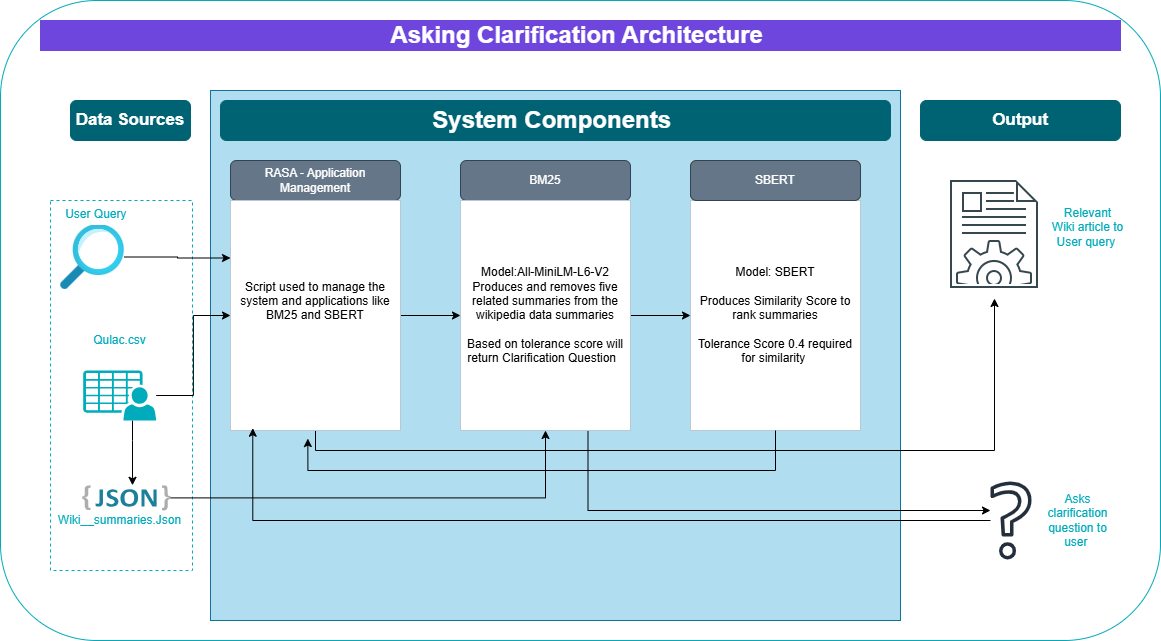
\includegraphics[width=\linewidth]{./img/system_diagram.png}
  \caption{System Diagram for our Clarification project}
  \label{fig:sys_diag}
\end{figure}

\subsection{Qulac Dataset}
The Qulac - short for Questions for Lack of Clarity—is a benchmark dataset created to support research on asking clarifying questions in open-domain, information-seeking conversations and was one of the primary datasets for this system. One of the initial steps was to appropriately shape the data to work with the other elements within our system. The transformations for cleaning this dataset were performed initially in Python using the Pandas library, and the resulting CSV was stored within GitHub.

\subsection{Original Qulac Dataset}
In short the Qulac dataset is a dictionary with query keys and a list of relevant facet descriptions (user intents).

Each query in Qulac is paired with a set of ten candidate clarifying questions, which are designed to resolve potential ambiguity. For example, the query "jaguar" could relate to the animal, the car brand, or even the sports team, and Qulac includes questions such as “Are you referring to the animal or the car brand?” to help systems distinguish between these interpretations. These questions were manually authored and assessed through crowdsourcing to ensure relevance and effectiveness in eliciting more specific user intent. Queries are also accompanied by retrieved web passages from the ClueWeb09 Category B corpus, providing context for question evaluation.

The dataset includes annotations from human judges who rated each candidate question based on its helpfulness, relevance, and clarity. The ratings fall into categories such as excellent, good, fair, or bad, offering a rich signal for training supervised learning models. These annotations allow for the creation of ranking systems that prioritize better clarifying questions over less helpful ones. The inclusion of such human judgments positions Qulac as a valuable dataset for evaluating both neural ranking models and question generation systems in the conversational IR domain.

\subsection{Clean Qulac Schema}
\renewcommand{\arraystretch}{1.2} % increase row height for readability

\begin{table}[ht]
  \centering
  \caption{Transformed Qualac Dataset for BM25 and Wiki Summaries}
  \label{tab:dataset-columns}
  \begin{tabularx}{\columnwidth}{@{} l l X @{}}
    \textbf{Column Name}  & \textbf{Type}    & \textbf{Description}                        \\ 
    \hline
    Index                 & String           & Facet index based on word string.            \\ 
    Category Name         & String           & Name of the broader category of the dataset. \\ 
    Facet Description     & String           & Detailed description of the facet.           \\ 
    Col 1                 & String           & Response 1.                                  \\ 
    Col 2                 & String           & Response 2.                                  \\ 
    Col 3                 & String           & Response 3.                                  \\ 
    Col 4                 & String           & Response 4.                                  \\ 
    New Index             & Integer          & Row index counter.                           \\ 
  \end{tabularx}
\end{table}

One of the most important features of the Qulac Dataset was the facet descriptions, as they were used to derive the Wikipedia Summaries. A facet is a clarifying intent subtopic to given a query. Let us take "Cat" as an example of a facet. In this scenario there are four potential facets for cats; the mammal - felius catus - , the musical  and the shoe brand. The facet description are important as they give meaning and context when searching for the correct wikipedia. Hence they important for deriving the correct wikipedia summaries. 

\subsection{Wikipedia Summaries}
The Wikipedia summaries were generated using a series of GET responses contained within a Python script on the Wikipedia API. The aim was to generate five summaries per topic based on the facet descriptions \textendash{} relating to the user's query. In short, the facet descriptions were used within a search function as to return the most relevant results within a given context. The reason why five results where generated instead of all possible results was to reduce the amount of noise in our dataset. Only the Wikipedia summaries where used to save on performance and time. In a larger and more extensive project, the entire Wikipedia summary should be generated. 

The method was crafted to ensure that it could retrieve data from the API at ease. If the project was larger in scope, the parameters and a couple of variables could be simply changed to gain the entire wikipedia article. 

Once completed, the Wikipedia Summaries were shaped into the cleaned dataset above. These summaries were required for BM25 later in the project. In a larger project, the Wikipedia API could be used to return the entire articles, but this would come at a cost of time, compute, and complexity.

\subsection{{RASA}}
RASA is the machine learning framework used for building this system. It is used to manage the dialogue by deploying the suitable modules. For this project, RASA deploys BM25 and SBERT, allowing the system to function cohesively. 

\subsection{Best Matching 25 (BM25)}
BM25 was a key ranking function used in the project for informational retrieval within the project. For the project, BM25 ranked the user queries to the relevant Wikipedia summaries giving them a ranking score. This function was imported from Huggingface via a python script. 
 \newline
 \newline
The documents used were the Wikipedia Summaries from the generated CSV. A ranking was also performed using all-MiniLM-L6-v2 from HuggingFace to select the best matching summary.

\subsection{SBERT}
The final step was determining the suitability of the top-ranked question. A specialised version of BERT called SBERT from Huggingface was utilised.

Our SBERT model was fine-tuned on \texttt{sbert\_training\_data.csv}, which contained two features: context and question. Each context is a formatted string combining the initial query and the next element. The model would try to find a similarity between the two strings to rank the relevant results.


\section{Evaluation}
\subsection{Rasa}
Rasa is an open-source conversational AI framework used to build context-aware chatbots. The core functionality of Rasa revolves around understanding user input, identifying their intent, and extracting relevant information, which is crucial for providing appropriate responses. 

When a user inputs a query, Rasa's NLU pipeline processes the message through several stages, including text preprocessing (tokenization, lowercasing, and punctuation removal). After preprocessing, Rasa uses a machine learning model to classify the intent behind the user's message. This model is trained on labelled data where various intents, such as “cheap\_internet” or “fickle\_creek\_farm” are predefined.

Entity extraction identifies key information within the message, such as dates or locations. Rasa then assigns a confidence score to each predicted intent, ranking them based on the similarity to the user input. If the confidence score is below a threshold, Rasa triggers clarification questions to gather more information, either by asking the user directly or using models like SBERT to rank and select the most relevant clarification question.

Once the intent and entities are determined, Rasa performs the necessary actions, which may include triggering predefined responses or custom actions, such as API calls. The system then responds to the user with the appropriate answer, either static or dynamically generated.

Overall, Rasa's intent recognition process combines machine learning and NLP to handle user input, enabling a seamless and interactive chatbot experience.

\subsection{BM25}
To understand the effectiveness and behaviour of the BM25 and all-MiniLM-L6-v2 retrieval pipeline, a three-part evaluation was designed. 150 queries were generated using GPT-4 (reference) to test on the model and produce statistics on its performance. These queries were split into the following three categories:
\begin{enumerate}
\item Matching queries - 50 queries based on content that appears in the dataset, each paired with a “ground truth” summary. The ground truths were the summaries that best answered the queries according to GPT-4 \cite{OpenAI2025}. For example: “What is The North Island brown kiwi?”
\item Non-matching queries - 50 queries that had nothing to do with the dataset. These did not feature ground truth, as they were designed to lack a satisfying answer in the partition of the Qulac dataset used in the pipeline \cite{Aliannejadi2021}. For example, “Who won the first season of The Voice?”
\item Ambiguous queries - 50 queries that were generalisations of topics related to summaries in the dataset but not directly answerable easily. For example, “Tell me about famous political figures.”
\end{enumerate}

All queries were run through the full BM25 and all-MiniLM-L6-v2 pipeline \cite{Brown2022,Tomaarsen2025a}. In the case of the 50 matching queries, the summary chosen by the pipeline was compared against the ground-truth using semantic similarity with \texttt{util.cos\_sim} \cite{Tomaarsen2025b}. If the similarity between the model's summary and the ground truth summary was greater than or equal to 0.7, the retrieval was considered successful. This allowed for instances where there were two or more suitable summaries available in the dataset for a given query. Additionally, classification metrics were computed. Confident predictions were treated as positive predictions, and semantic matches defined correctness.

\subsection{SBERT}
To evaluate the performance of our fined-tuned SBERT model the ranking of clarification question \cite{Tomaarsen2025b}. A custom dataset of 75 ambiguous queries.  is created with GPT. These are diverse set of queries spans a wide varieties of topics like technology, environment, health, education, finance psychology and more to test the models semantic flexibility and its ability to generalise beyond its familiar domain. Each query was paired with their four candidate clarifying questions. Out of which one was the most contextually appropriate.  The model was tested to see if I it could come up with the most contextually appropriate follow up and that it understands the intent of the query or not. 

The model used is a fine-tuned version of the all-MiniLM-L6-v2, it is a compact SBERT model producing 384-dimensional sentence embeddings which was pretrained for ranking clarifying questions by understanding the intent \cite{Tomaarsen2025a}. During fine-tuning the model was trained on 196 positive Query-clarification pairs from the Qulac dataset using the MultipleNegativesRankingLoss \cite{Tomaarsen2025c}. This setup enabled the model to rank multiple clarifications for a single query, which makes it ideal for retrieval and dialog system like RASA. 

The aim of the evaluation is measuring model's semantic understanding, confidence behaviour, and it's overall suitability for a real-time integration into a retrieval-based dialog system. The performance was measured primarily through cosine similarity scores and confidence thresholds to determine how well the model aligned clarifications to the query intent.
Basically, the evaluation assesses whether the model can rank the best clarification for each query and also understand user intent, especially in ambiguous scenarios. A confidence threshold of 0.40 is defined on cosine similarity to judge the reliability of the model's top choice.


\section{Results and Discussion}
\subsection{BM25}

\begin{table}[t]
  \centering
  \begin{tabular}{lr}
    \textbf{Metric} & \textbf{Value} \\
    \hline
    Accuracy & 92.00\% \\
    Precision & 100.00\% \\
    Recall & 91.49\% \\
    F1 Score & 95.56\% \\
    Avg. cosine sim. & 0.5882 \\
    Avg. semantic sim. & 0.9594 \\
  \end{tabular}
  \caption{Performance metrics for matching queries.}
  \label{tab:matching-metrics}
\end{table}

The results shown in \autoref{tab:matching-metrics} indicate strong metrics across the board, particularly in precision, meaning the system was never confidently wrong. However, it occasionally failed to respond confidently even when it should have as seen by the slightly lower recall. This suggests the pipeline was cautious yet reliable.
To comment on the logic used to compute these statistics, the definitions illustrated in \autoref{tab:classification-definitions} were coded into the evaluation script.

\begin{table}[t]
  \centering
  \begin{tabular}{p{0.50\linewidth}p{0.38\linewidth}}
    \textbf{Behaviour} & \textbf{Term} \\
    \hline
    Confident, sim. $\geq$ 0.7 & True Positive (TP) \\
    Confident, sim. $<$ 0.7 & False Positive (FP) \\
    Not confident, sim. $\geq$ 0.7 & False Neg. (FN) \\
    Not confident, sim. $<$ 0.7 & True Neg. (TN) \\
  \end{tabular}
  \caption{Classification definitions.}
  \label{tab:classification-definitions}
\end{table}

To calculate the evaluation metrics, the code presented in \autoref{fig:eval-metrics-code} was used.

\begin{figure}[t]
  \centering
  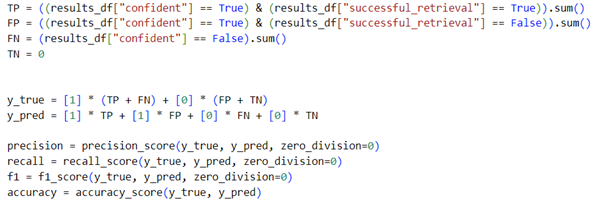
\includegraphics[width=\linewidth]{img/eval_metrics_code.png}
  \caption{Evaluation metrics calculation code.}
  \label{fig:eval-metrics-code}
\end{figure}

It should be noted that True Negatives were set to 0 as every query had a correct associated answer, meaning that there could be no True Negatives for the matching queries. 

As for the ambiguous queries, the results shown in \autoref{tab:ambiguous-query-results} were produced.

\begin{table}[t]
  \centering
  \begin{tabular}{l r}
    \textbf{Metric} & \textbf{Value} \\
    \hline
    Confident predictions & 42\% \\
    Avg. cosine similarity & 0.3584 \\
  \end{tabular}
  \caption{Ambiguous query results.}
  \label{tab:ambiguous-query-results}
\end{table}

In this case, the model was appropriately hesitant. The low average demonstrates that even when the pipeline attempted an answer (which happened 42\% of the time), the fit was often poor (0.3584 average cosine similarity), which supports the system's ability to avoid overconfident guessing where the model is not sure. 

As for the non-matching queries, the metrics seen in \autoref{tab:nonmatching-metrics} were calculated.

\begin{table}[t]
  \centering
  \begin{tabular}{l r}
    \textbf{Metric} & \textbf{Value} \\
    \hline
    Correctly cautious (not confident) & 80\% \\
    False positives (wrongly confident) & 20\% \\
    Avg. cosine similarity & 0.2839 \\
  \end{tabular}
  \caption{Metrics for non-matching queries.}
  \label{tab:nonmatching-metrics}
\end{table}

This indicates the system could not answer 80\% of irrelevant queries, which is desirable when compared to matching and ambiguous queries. However, the 20\% false positive rate means the system attempted to answer one in five queries, even when no relevant summaries existed. This is disappointing, but relatively fine compared to the confidence scores from the other query groups (92\% and 42\% respectively).

Ultimately, the evaluation of the retrieval pipeline was robust, and highlighted the success of the model. However, it was not possible to implement Precision, Recall, and F-1 scores for the ambiguous and non-matching query groups, as ground truths were impossible to even synthetically produce due to the nature of the groups. Ideally, comparing the model's results against the results of a perfect model would be the best evaluation method, but the task is to subjective to expect perfection from any pipeline. The drops in accuracy and cosine similarity as the model transitioned from matching, to ambiguous, to non-matching do represent a solid evaluation architecture though, and suggest the pipeline performance was more than capable of performing summary retrieval where fit for any given query.

\subsection{SBERT}
All the 75 ambiguous queries were passed through the trained SBERT model, and the cosine similarity were computed between the query and associated clarifying questions. And the resultant clarification with the highest score was selected as the top prediction made by the model. The prediction is only considered as “confident” if the top similarity score $\geq$ 0.40 threshold.

\begin{table}[h]
  \centering
  \begin{tabular}{l r}
  \textbf{Metric} & \textbf{Results} \\
  \hline
  Total Queries & 75 \\
  Confident predictions ($\geq 0.40$) & 63 (84\%) \\
  Not confident & 12 (16\%) \\
  Avg. cosine similarity score (TOP) & 0.563 \\
  Avg. cosine (non-confident) & 0.38 \\
  \hline
  \end{tabular}
  \caption{SBERT prediction confidence and similarity metrics}
  \label{tab:sbert-results}
\end{table}
  
The metrics and results used are displayed in \autoref{tab:sbert-results}. The standard metrics like Precision, re-call and f1 score were not used, as this is a ranking task, not a binary classification task with negative labels.

The SBERT model demonstrated a strong semantic understanding capability in confidently ranking the contextually appropriate clarification where the ambiguous queries were diverse and different from the original Qulac data the model was trained on. The 84\% confident score and the 0.563 percent of average similarity shows that the model capable and it is understanding the semantics of the Query-clarification of a new diverse dataset. Also mentioning that the queries in which the model was not confident the average of similarity is around decision threshold. (0.38) which indicate the model's ability to express it uncertainty when there is less semantic alignment. This reduces the risk of returning irrelevant clarifications.  Reduces the chances of overconfident incorrect responses.

Although the model is good at expressing any uncertainties, but it sometimes refrains from answering even when a reasonably close clarification exists.  This behaviour can limit the system's responsiveness in the practical deployment.
The clarification is more subjective and contextual unlike the summary retrieval task. The subjectivity and context sensitive makes it harder to evaluate the model's performance using the standard classification metrics or generate ground truth labels. This lack of having ground truth can introduce some ambiguity in the interpretation of the results and tuning threshold.  This can be improved by training a model to a larger dataset and it can be finetuned for a particular domain-specific clarification task as well can be trained on a large amount of diverse data to increase the accuracy of the results overall.


\section{Conclusion}
Ultimately, this project successfully demonstrated a functional conversational search system that takes user queries as input, and outputs clarifying questions or satisfactory wiki summaries. By combining a retriever model (BM25) with a semantic reranker (all-MiniLM-L6-v2) to form a comprehensive summary retrieval pipeline, and a fine-tuned SBERT model for clarification questions, the system was able to deliver relevant responses or appropriate follow-up questions to the user. These interactions were handled through the Rasa dialogue manager, which acted as a middleman ensuring smooth conversational flow and intent management.

Evaluation results showed that the retrieval pipeline achieved strong performance on matching queries (92\% accuracy, 95.56\% F1 score, and 0.9594 average semantic similarity). This confirmed its effectiveness in returning relevant summaries when sufficient information was provided. On ambiguous queries, the system produced confident predictions only 42\% of the time with a lower average similarity of 0.3584, thus demonstrating excellent uncertainty handling. For non-matching queries, the system was correctly cautious in 80\% of cases.

The SBERT clarification handling also showed promising results, ranking the correct question with confidence 84\% of the time, with an average similarity of 0.563 across 75 queries of differing nature. It also showed its ability to give uncertainty (12 queries below the confidence threshold) which, supports expected behaviour in ambiguous contexts.

A key component enabling the system's interactivity was the Rasa dialogue manager. Rasa handled user input, tracked conversation history, and coordinated the conversational flow between the user and the model seamlessly. Rasa helped the system mimic real conversational behaviour, therefore making it an apt tool for managing interactive search.

Although limiting factors such as the size of the dataset sourced from the Qulac dataset, and the fixed set of clarifying questions constrained the system's general ability somewhat, the pipeline still proved effective within its scope.  Additionally, the SBERT model was only fine-tuned on a small subset of the data, which may have lessened its ability to generalise across rare query types. Fundamentally however, the system achieved its primary goal: to decide when clarification is needed and deliver either a relevant summary or an appropriate clarifying question. Within a lightweight framework, it demonstrated reliable performance and the potential for real-world applicability in conversational search.

\subsection{Future Work}
In terms of future work, the primary objective should be to broaden the scope and foundation of the current project and address the issues identified in the limitations:

\begin{itemize}
    \item \textbf{Investigate and implement methods for generating clarifying questions for the system.} The current system has difficulty in clarifying many questions, and having a larger dataset of facets would improve its efficiency.
    
    \item \textbf{Replace the Wikipedia summaries with a system that directly responds to users' queries.} This would necessitate the implementation of Retrieval-Augmented Generation (RAG), which was omitted from this project due to time constraints and complexity.
    
    \item \textbf{Conduct significantly more extensive research into other systems.} Although research was conducted, the range of areas investigated was limited. Future studies should expand the scope of research for the project and incorporate any findings within the field.
\end{itemize}

For any future research to be successful, it will need to provide more optimal timelines and expertise to effectively implement the aforementioned points.


\section*{Limitations}
While our system has met the main project requirements, including asking clarifying questions during conversations, selecting clarifying questions, and evaluating a clarifying question-answering system, there are several limitations worth discussing:

\begin{itemize}
    \item \textbf{The selection of questions for clarification.} Our system uses curated questions from the Qulac dataset to train our data, which helps streamline report production and meet deadlines but does not fully replicate real-life scenarios.
    
    \item \textbf{The use of Wikipedia summaries.} This approach may not completely satisfy end-user requirements. Users might prefer the entire Wikipedia article or just a brief sentence instead of a summary. The project focused on identifying and asking clarifying questions rather than the output, hence considering it less critical to meet this potential requirement. Consuming summaries was also easier to manage in terms of data quantity and system performance. Using entire articles would have posed challenges in storage and computation.
    
    \item \textbf{Research.} Although research informed the project's construction, no new discoveries were made in the field, indicating a lack of significant innovation in implementing this type of system.
\end{itemize}

Despite these limitations, given the nature of the project, time constraints, and available technical expertise, this solution is likely the most optimal that could be achieved within the given timeframe.


\section*{Ethics Statement}
This project developed a conversational search system for educational demonstrative purposes. All datasets used were publicly available and no personal, sensitive, or specific user data was collected or processed. As the system operates using predefined Wikipedia summaries and clarifying questions, the risk of harm to individuals or groups is minimal. 


\bibliographystyle{acl_natbib}
\bibliography{references}

\end{document}
